%
\subsection{Magnetic perturbations}
%
The magnetic perturbation from a TIEGCM model run can be determined
by using the postprocessor program \src{MagIon}. The program is available
upon request together a \src{MagIon} user guide, a model description
is in preparation. The global magnetic perturbations
at the ground and above the ionosphere at low orbiting satellite heights
can be determined, 
or what a magnetometer would measure at the ground. 
For details about the calculation and the
necessary assumption we refer to  \cite{rich74} and the 
\src{MagIon} user guide. \\

%
To calculate the magnetic perturbation the radial component of the field-aligned current
$J_{qr}$ and the height--integrated current densities $K_{m \phi}$
and $K_{m \lambda}$ have to be known. In addition, if the influence of 
gravity and plasma
pressure gradient driven current
should be included the height dependent $K_{m \phi}^{int}$
have to be determined with and without the current driven by gravity and plasma
pressure gradient. The calculation of these currents
is not the default in the TIEGCM source code, thus the flag  \flags{icalkqlam == 1} 
in the \src{module dynamo} has to be set. In the following the
calculation of the different currents $J_{qr}$, $K_{q \phi}$ and $K_{q \lambda}$, 
which can be found in the file \src{current.F}, is described. 
%
\subsubsection{Field--aligned current $J_{qr}$}\label{chap:jqr}
% 
The field--aligned current can be determined from the electrodynamo
equation (\ref{eq:edyn}) without the assumption of symmetrical
hemispheres which leads to 
%
\begin{equation}
 \begin{split}
  & \frac{\partial}{\partial \phi_m} \bigl( \frac{\Sigma_{\phi \phi}}{cos
   \lambda_m} \frac{\partial \Phi}{\partial \phi_m} + 
   \Sigma_{\phi \lambda} \frac{\partial \Phi}{\partial |\lambda_m|} \bigr) +
   \frac{\partial}{\partial | \lambda_m |} \bigl( \Sigma_{\lambda \phi}
    \frac{\partial \Phi}{\partial \phi_m} + 
   \Sigma_{\lambda \lambda} cos \lambda_m 
   \frac{\partial \Phi}{\partial |\lambda_m|} \bigr) \\
  &  =
   R \frac{\partial K_{m \phi}^{D}}{\partial \phi_m} +  
   R \frac{\partial K_{m \lambda cos \lambda_m }^{D}}{\partial | \lambda_m |} +
   R^2 cos \lambda_m J_{mr}
    \label{eq:edyn_wosym}
  \end{split}
\end{equation}
%
Note that compared to the electrodynamo equation (\ref{eq:edyn}) the
conductances and the wind driven current are different in the northern and
southern hemisphere denoted by e.g. $\Sigma_{\phi \phi}$ instead of 
$\Sigma_{\phi \phi}^T$. Therefore we determine the finite difference coefficient 
stencil for both
hemispheres instead of only one as described in section \ref{chap:finitediff} on
page \pageref{page:diff_lhs}. The set up of the finite difference stencil  
is analog to the one for only one
hemisphere. The  \src{subroutine nosocoef} sets up the
coefficient stencil for both hemisphere and also saves the wind driven current.
The  \src{subroutine nosocoef} is called shortly after the field line
integrations i.e. before the conductances and wind driven currents are added
together from the two hemispheres (see table \ref{tab:transf_quantities}). 
The conductances are prepared for the finite differencing
and represent 
% 
\begin{align}
A=& \frac{\Sigma_{\phi \phi}(0)}{cos\lambda_0  \Delta \phi^2 }	   \rightarrow  nszigm11\label{eq:nssig_dif1}\\
B=& \frac{\Sigma_{\lambda \lambda}^(0) cos \lambda_0}{\Delta \lambda_0^2} \rightarrow  nszigm22\label{eq:nssig_dif2} \\
C=& \frac{\Sigma_{\phi \lambda}(0)}{4\Delta \lambda_0 \Delta \phi }    \rightarrow  nszigmc \label{eq:nssig_dif3} \\
D=& \frac{\Sigma_{\phi \lambda}(0)}{4 \Delta \lambda_0 \Delta \phi}    \rightarrow  nszigm2 \label{eq:nssig_dif4} 
\end{align}
%
The set up of the stencil is analog to section \ref{chap:finitediff}
see table \ref{tab:stencil} and \ref{tab:stencil_eq} with A, B, C and D
from the definitions above eq. (\ref{eq:nssig_dif1})--(\ref{eq:nssig_dif4}). \\

The calling tree is 
%
\begin{verbatim}
...
call nsstencil
   call nscnm
...
\end{verbatim}
%
Note that the stencil is only calculated on the finest grid. In addition
no  upwinding method to preserve the diagonal dominance is used  
since the finite difference stencil is not used for solving. The numbering
 of the nine node stencil for the
southern hemisphere is the same as for the northern hemisphere, which is illustrated in 
 figure \ref{fig:nsstencil} for both hemispheres. This means that e.g. points 6'', 7'' and 8'' 
in the southern hemisphere are toward the poles and not toward the equator as for the northern hemisphere
points 6, 7 and 8.
This switch of the nodes 6, 7, 8 with 4, 3, 2 is reflected in the set up
of the stencil in the southern hemisphere done in \src{subroutine nscnm}.
The result is stored in the array \src{nscoef}. The wind driven currents
of the right hand side are treated in the same way as in the dynamo
equation in section  \ref{chap:finitediff} on page \pageref{page:finite_rhs}.
The right hand side is saved in the array \src{nsrhs}.
 \\
 
%
\begin{figure}
  \centering
  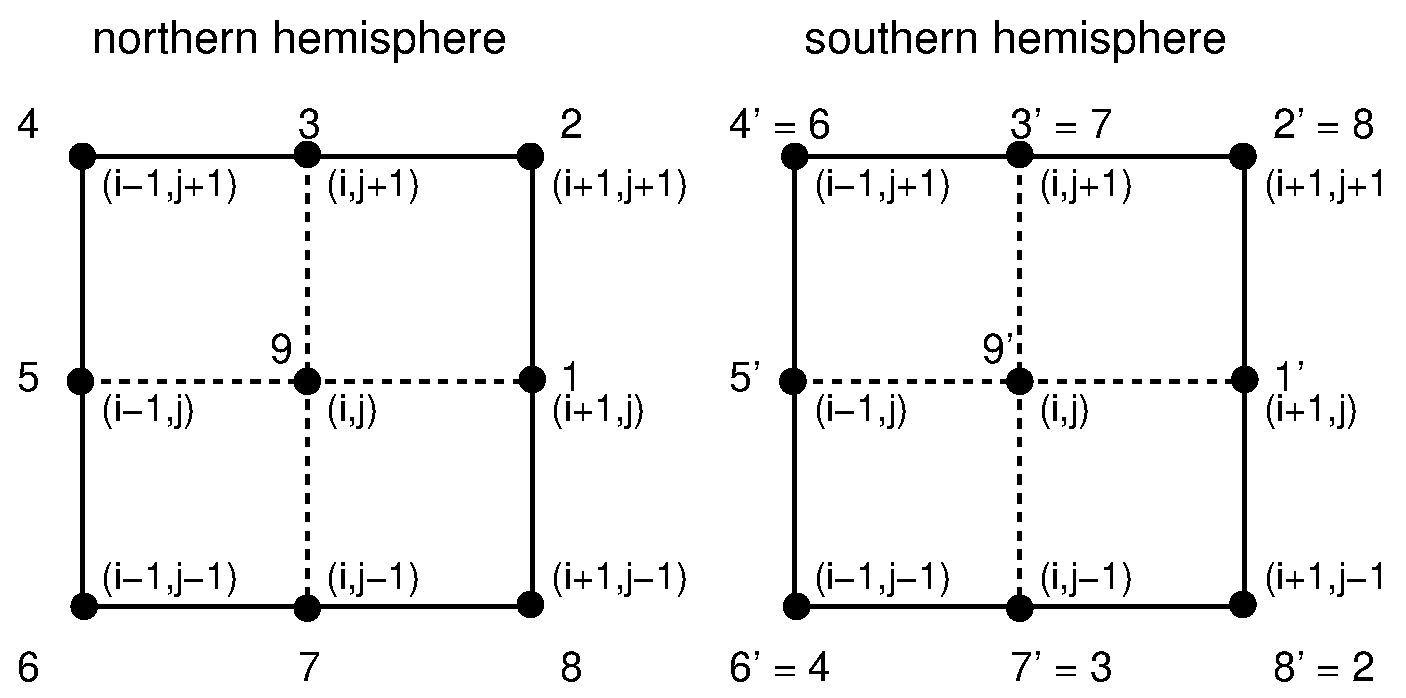
\includegraphics[scale=0.5]{./tex_plot/ns_stencil.eps}
  \caption{Geometry for the 9 point stencil in the northern and southern hemisphere}
   \label{fig:nsstencil}
\end{figure}
%

Having set up the finite difference coefficient matrix $\bar{\mathbf{C}}$ of the 
left hand side, as described
in the previous paragraph, and determined the wind driven current of the right
hand side vector $\mathbf{rhs}$ we can insert the 
calculated electric potential vector $\mathbf{\Phi}$ 
into equation
(\ref{eq:edyn_wosym}) to solve for the field aligned current vector $\mathbf{J}_{mr}$.
%
\begin{equation}
   R_0^2 \frac{cos \lambda_m}{cos \lambda_0}
  \frac{\partial \lambda_0}{\partial \lambda_m^*} J_{mr} = \bar{C} \Phi - \text{rhs} \label{eq:jmr_solve}
\end{equation}
%
Note that the whole electrodynamo equation was multiplied by
$\frac{1}{cos \lambda_0}\frac{\partial \lambda_0}{\partial \lambda_m^*}$ as mentioned 
on page \pageref{page:electro_multi}. The current calculation is done
in \src{subroutine nosocrrt}. For the polar values the average values at
adjacent latitudinal point are extrapolated by
%
\begin{align}
  J_{mr} (j_{pole})= & \frac{1}{8 \text{nmlon}} \bigl[ 
     9\sum_{i=1}^{nmlon} {J}_{mr} (i,j_{pole} \mp 1)
    - \sum_{i=1}^{nmlon} {J}_{mr} (i,j_{pole} \mp 2)\bigr] 
\end{align}
%
with $nmlon$ the number of longitudes and $j_{pole}$ the latitudinal index at
the north / south pole and the $\mp$ sign referring to the poles
respectively. 
Close to the magnetic equator there is no distinct allocation of the
current to either the height integrated current density $K_{m \lambda}$
or the field--aligned current $J_{mr}$ since the magnetic field lines are
almost horizontal in this region. Therefore the allocation to either one of 
the two currents $K_{m \lambda}$ and $J_{mr}$ depends strongly on the 
reference height $h_0$. Raising the reference height will shift the current 
from the field line to the ionospheric current sheet $K_{m \lambda}$. The 
exact distribution of the current at the equator can be neglected for the
calculation of the magnetic perturbations. Therefore we linearly interpolate 
the field--aligned current between $\pm 12^o$ latitude.
%
\begin{align}
  J_{mr} (j)= \frac{J_{mr}(\lambda_m^{max}) J_{mr}(\lambda_m^{min}) }
  {\lambda_m^{max} - \lambda_m^{min}} (\lambda_m-\lambda_m^{min}) 
  + J_{mr} (\lambda_m^{min}) & \\
    \quad \text{for} \quad \lambda_m^{min} \leq \lambda_m \leq \lambda_m^{max} &
\end{align}
% 
with $\lambda_m^{min} = -12^o$ and $\lambda_m^{max} = 12^o$. 
Due to the linear interpolation at each latitude
higher frequency modes are introduced which are smoothed by a weighted
average in longitude.
%
\begin{align}
  J_{mr} (j)= \frac{1}{5} [J_{mr}(i+1,j) + 3 J_{mr}(i,j) + J_{mr}(i-1,j)  ]
\end{align}
% 
Since the field--aligned
current $J_{mr}$ is used to calculate the ionospheric equator-- / 
downward current sheet contribution
 $K_{m \lambda}$ the total current system
 is adjusted automatically to satisfy that it is divergence free.
 
%
\subsubsection{Eastward current $J_{e1}$ and height integrated current densities
 $K_{q\phi}$, $K_{q\lambda}$}
% 
To calculate the eastward height integrated current density $K_{q \phi}$, see also
eq. (7.4) in \cite{rich95},
%
\begin{align}
  K_{q \phi} = \int_{h_l}^{h_u} \bigl(\frac{R_E+h}{R_0}\bigr)^{5/2} \frac{J_{e1}}{F} dh
  \label{eq:kmphi_1}
\end{align}
% 
the eastward current $J_{e1}$ has to be known. The eastward current $J_{e1}$ is
determined by, see also
eq. (5.7) in \cite{rich95},
%
\begin{align}
  \frac{J_{e1}}{D} = \sigma_P \frac{d_1^2}{D}(E_{d1} + u_{e2}B_{e3}) + 
      (\sigma_P \frac{\mathbf{d}_1 \cdot \mathbf{d}_2}{D} - \sigma_H)
      (E_{d2} - u_{e1}B_{e3}) + \text{fac} \frac{J_{e1}^{p,g}}{D}
\end{align}
% 
The downward--/ equatorward current component $J_{e2}$ is only calculated for postprocessing
reasons.
%
\begin{align}
  \frac{J_{e2}}{D} = \sigma_P \frac{d_2^2}{D}(E_{d2} - u_{e1}B_{e3}) + 
      (\sigma_P \frac{\mathbf{d}_1 \cdot \mathbf{d}_2}{D} + \sigma_H)
      (E_{d1} + u_{e2}B_{e3}) + \text{fac} \frac{J_{e2}^{p,g}}{D}
\end{align}
%
with $\text{fac}=10^4$ being the conversion factor from $\frac{1}{cm^2}$ to $\frac{1}{m^2}$. 
The current components are computed on the half pressure levels. The input
quantities $\sigma_H$, $\sigma_P$, $\frac{d_1^2}{D}$, 
$\frac{\mathbf{d}_1 \cdot \mathbf{d}_2}{D}$, $u_{e1}$, $u_{e2}$ and $B_{e3}$ are
all stored at half pressure levels. Only the electric field $E_{d1}$ and $E_{d2}$
are at full pressure levels and have to be converted to half levels by
%
\begin{align}
   E_{d1}(k') = \frac{1}{2} (E_{d1}(k) + E_{d1}(k+1) )
\end{align}
% 
with k' denoting the half pressure level index $k' = k+ \frac{1}{2}$. We assume that
$\frac{d_2^2}{D} =1$ everywhere which is approximately true. In addition to this
simplification the height variation of the magnetic field component $B_{e3}$
is neglected. The current contribution due to plasma pressure gradient and gravity 
$J_{e1}^{p,g}$ is
%
\begin{align}
  \frac{J_{e1}^{p,g}}{D} = \frac{\mathbf{J}_{p}\cdot \mathbf{d}_1 + 
          \mathbf{J}_{g}\cdot \mathbf{d}_1}{D}  
\end{align}
% 
with $\mathbf{J}_{p}$ determined in section \ref{subsec:ppres_current}  by
eq. (\ref{eq:j_p}) and the gravity term  $\mathbf{J}_{g}$ in section 
\ref{subsec:grav_current} by eq. (\ref{eq:j_g}). The gravity and plasma pressure 
gradient current is calculated in \src{subroutine magpres\_grav} on the
geographic grid and is mapped afterward to the geomagnetic grid. Both terms $\mathbf{J}_{p}$
 and $\mathbf{J}_{g}$ are stored at half pressure levels. \\
 
Once the eastward current $J_{e1}$ is determined the height integrated
eastward current density $K_{m \phi}$ can be calculated by using eq. (\ref{eq:kmphi_1})
with the dipole filed quantity
 $F$ quantity, see also eq. (6.9) in \cite{rich95},
%
\begin{align}
  F = \frac{sin \lambda_m}{sin \lambda_q}\frac{sin I}{sin I_m}\bigl(\frac{R_E+h}{R_0}\bigr)^3 D
  \label{eq:kqphi_f} 
\end{align}
% 
Inserting eq. (\ref{eq:kqphi_f}) into eq. (\ref{eq:kmphi_1}) leads to
%
\begin{align}
 K_{q \phi} = \int_{h_l}^{h_u} \frac{J_{e1}}{D} 
 \frac{sin \lambda_q}{sin \lambda_m}\frac{sin I_m}{sin I}\bigl(\frac{R_0}{R_E+h}\bigr)^{1/2} dh
  \label{eq:kqphi_insert} 
\end{align}
% 
which is calculated at full pressure levels. The height integrated current densities are
calculated assuming a dipole field which is indicated by the index $(\cdot)_q$ of
$K_{q \phi}$. Therefore the height integration is done in height rather than along
the field line. The difference between height and field line integration at mid--
and high latitude is small since the field lines are almost vertical through
the ionospheric current sheet. 
The dipole latitude $\lambda_q$ in 
eq. (\ref{eq:kqphi_insert}) is
%
\begin{align}
 sin \lambda_q (h) = sin \lambda_m (h_0)
\end{align}
% 
We assume dipolar field lines such that $\lambda_m (h)$ can be computed by
%
\begin{align}
 cos^2 \lambda_m (h) = \frac{R_0}{R} cos^2 \lambda_q
\end{align}
% 
The sinus of the inclination angle $I_m$ is determined by
%
\begin{align}
  sin I_m = \frac{2 sin \lambda_m(h_0)}{\sqrt{1 + 3 sin^2 \lambda_m(h_0)}}
\end{align}
% 
and the sinus of the angle $I$ by
%
\begin{align}
  sin I = \frac{B_z}{|B_0|}
\end{align}
% 
with $|B_0|$ the magnitude of the geomagnetic field and $B_z$
the downward component. Note that we assume that both quantities vary
in the same way in height and therefore no height variation is taken
into account. The equatorial values of $ sin I $ and $sin \lambda_q$
are taken from the adjacent grid point in latitude. The height integral
is the sum over all height levels with
%
\begin{align}
  K_{q \phi} = \sum_{k=-2}^{\text{mlev}} S(k') 
    J_{e1}(k') dh(k) \label{eq:kqphi_total}
\end{align}
% 
with $J_{e1}(k')$ the eastward current at the half pressure level between k and k+1.
The term S denotes $\frac{sin \lambda_q}{sin \lambda_m}\frac{sin I}{sin I_m}
(\frac{R_0}{R_E+h})^{1/2}$ which is known at the full level e.g. k and k+1
and therefore has to be interpolated to the half pressure level. 
The discrete height
$dh$ is determined by $dh = \frac{1}{100} [z(k+1) - z(k)]$ in [m]. \\
%
For the
calculation of the magnetic perturbations due to plasma pressure gradient and
gravity driven current, the height distribution of the eastward current density denoted by 
$K_{m \phi}^{int}$ has to be known. The previous assumption that most of the current is
flowing in a thin current shell is not valid anymore since the current due to
gravity and plasma pressure gradient is flowing in the E-- and F--region.
Therefore the height dependent current density at pressure level $k^*$ is
calculated by
%
\begin{align}
  K_{m \phi}^{\text{int}}(k^*) = \sum_{k=-2}^{k^*} S(k')
    J_{e1}(k') dh(k)\label{eq:kqphi_int}
\end{align}
% 

%
Once the height integrated eastward current density $K_{q \phi}$ and the radial
component of the field aligned current $J_{mr}$ are determined by equations 
(\ref{eq:jmr_solve}) and (\ref{eq:kqphi_total}) the height integrated northward
current density $K_{q \lambda}$ can be calculated such that the current system is
divergence free
%
\begin{align}
  J_{mr} = \frac{-1}{R cos \lambda_q} \bigl[ 
    \frac{\partial K_{q \phi}}{\partial \phi_q} + 
    \frac{\partial (K_{q \lambda} cos \lambda_q)}{\partial \lambda_q}  
    \bigr]\label{eq:jmr_div}
\end{align}
% 
Solving eq. (\ref{eq:jmr_div}) for the the height integrated northward 
current density $K_{q \lambda}$ leads to
%
\begin{align}
  K_{q \lambda} (\phi_q,\lambda_q^*)= - \frac{1}{cos \lambda_q^*} \int_{-\frac{\Pi}{2}}^{\lambda_q^*}
   \bigl[ J_{mr} R cos \lambda_q + \frac{\partial K_{q \phi}}{\partial \phi_q} 
   \bigr] d \lambda_q\label{eq:kmlambda}
\end{align}
% 
The derivative $\frac{\partial K_{q \phi}}{\partial \phi_q}$ is approximated by
central differencing
%
\begin{align}
   \frac{d K_{q \phi}(i,j)}{d \phi_q} = \frac{K_{q \phi}(i + \frac{1}{2},j) - 
   K_{q \phi}(i - \frac{1}{2},j)}{2 \Delta \phi_q} 
   \label{eq:deriv_kqphi}
\end{align}
%
with i being the longitudinal index and $i + \frac{1}{2}$ denoting the average
between the grid points i and i+1. We substitute the following term for
simplicity 
%
\begin{align}
   T(i,j) =  J_{mr}(i,j) R cos \lambda_q(j) + \frac{d K_{q \phi}(i,j)}{d \phi_q}
   \label{eq:kqlam_simpl}
\end{align}
%
into equation (\ref{eq:kmlambda}). The integration is done over the
southern and northern hemisphere separately since the total current in
both hemispheres has to cancel. 
%
\begin{align}
   S^{SH}(i,j^*) &= - \sum_{j=2}^{j^*} T(i,j-\frac{1}{2})[\lambda_j - \lambda_{j-1}]
    \quad \frac{nmlat+1}{2} \ge j^* > 2 \label{eq:kqlam_sum sh} \\
   S^{NH}(i,j^*) &=  \sum_{j=nmlat-1}^{j^*} T(i,j+\frac{1}{2})[\lambda_j - \lambda_{j-1}]
    \quad \frac{nmlat+1}{2} < j^* \le \text{nmlat-1} \label{eq:kqlam_sum_nh}
\end{align}
%
In addition the integral of the absolute northward current is computed by
%
\begin{align}
   | S^{SH}(i,j^*)| &= - \sum_{j=2}^{j^*} | T(i,j-\frac{1}{2})[\lambda_j -
      \lambda_{j-1}]|
    \quad  \frac{nmlat+1}{2}\ge j > 2 \label{eq:kqlam_abssum sh} \\
   | S^{NH}(i,j^*)| &=  \sum_{j=nmlat-1}^{j^*} | T(i,j+\frac{1}{2})[\lambda_j -
      \lambda_{j-1}] |
    \quad \frac{nmlat+1}{2} < j \le \text{nmlat-1} \label{eq:kqlam_abssum_nh}
\end{align}
%
The northward current $K_{q \lambda}$ has to be corrected to assure that the sum over
both hemispheres vanishes.  The magnitude of the correction $\epsilon^{SH}$ and
$\epsilon^{NH}$ for the two hemispheres is calculated at each longitude $\phi_q(i)$.
%
\begin{align}
   \epsilon^{SH}(i) = \frac{1}{2} \frac{S^{SH}(i,j^*) - S^{NH}(i,j^*)}{|S^{SH}(i,j^*)|}  | \quad 
   \text{with} \quad j^* = \text{nmlat}\label{eq:kqlam_epsilon_sh} \\
   \epsilon^{NH}(i) = \frac{1}{2} \frac{S^{SH}(i,j^*) - S^{NH}(i,j^*)}{|S^{NH}(i,j^*)|}  | \quad 
   \text{with} \quad j^* = \text{nmlat}\label{eq:kqlam_epsilon_nh} 
\end{align}
%
The corrected northward height integrated current densities in the southern and northern 
hemisphere are
%
\begin{align}
   K_{q \lambda}^{cor}(i,j) = \frac{1}{cos \lambda_q} [S^{SH}(i,j) - \epsilon^{SH}(i)
   |S^{SH}(i,j)|]\label{eq:kqlam_cor sh}
    \quad  \frac{nmlat+1}{2}\ge j > 2 \\
   K_{q \lambda}^{cor}(i,j) = \frac{1}{cos \lambda_q} [S^{NH}(i,j) + \epsilon^{NH}(i)
   |S^{NH}(i,j)|]
    \quad \frac{nmlat+1}{2} < j \le \text{nmlat-1} \label{eq:kqlam_cor nh} 
\end{align}
%
with the error $\epsilon$ distributed according to the weight of $|S(i,j)|= 
|K_{q \lambda}(i,j)|$. The eastward current $J_{e1}$, the height integrated
current densities $K_{q \phi}$ and $K_{q \lambda}^{cor}$, as well as the height
dependent current density $K_{q \phi}^{int}$ are all calculated in 
\src{subroutine nosocrdens}.
